\documentclass{proc}
\usepackage{graphicx}
\usepackage{mathtools}
\usepackage{fixltx2e}
\usepackage{algorithm}
\usepackage{algpseudocode}
\usepackage{caption}
\usepackage{url}
\usepackage{amsmath}
\usepackage{mathrsfs}
\usepackage{tikz}
\usetikzlibrary{positioning}
\setlength{\abovecaptionskip}{2pt}
\setcounter{secnumdepth}{2}

\title{
The Small World Network Effect in Open Source Project Teams
\author{Kevin Peterson\\
\small \texttt{pete1968@umn.edu}
}
}

\begin{document}
\maketitle

\begin{abstract}
Team cohesion and the dynamics of team forming are important parts of any project, with software projects being no exception. An interesting aspect of team building is the relationships formed between the team members. If follows that visualizing software team members as a graph can give some insight as to what the optimal team conditions are. As team members move between projects, these graphs gets more and more connected as team members make connections. We show that this connectivity, known as the "small world effect," has a positive impact on team performance at when the connectivity levels are moderate. This aligns with similar research findings of non-software teams. We do, however, find high performance at the extremes of the connectivity range.
\end{abstract}

\noindent \\\textbf{Keywords.} Git, GitHub, Open Source

\section{Introduction}
A social network is a graph people and the interactions between them. The dynamics of social networks have proved to be an important research topic for many different areas of study, from academic publication\cite{barabasi2002evolution}, to the success of broadway musicals\cite{uzzi2005collaboration}. In general, a social network is important to understanding how ideas and influence are spread\cite{kempe2003maximizing}, from which we can investigate the best conditions for optimal group perfomance within these networks.

A `small world' network is a social network characterized by high clustering of graph nodes paired with a short average path between nodes \cite{watts1998collective}. Milgram, in is seminal study, found that any two people are linked through a chain of friends and acquaintances on average of 6 people long\cite{milgram1967small}. From these observations, hypotheses can be made as to the efficiency of how knowledge is transfered in these groups\cite{latora2001efficient}. In this work, we investigate the `small world' phenomenon and how it relates to Open Source Project Teams.


\subsection{Hypothesis}

\textit{Open Source Project Teams will perform best at moderate levels of $Q$. This performance, measured by the number of interest their projects generate, will increase as the level of $Q$ increases for the developer graph. This will continue up to an optimal $Q$ value, after which performance will begin to degrade. Thus, the performance curve given $Q$ will be U-shaped, and match Uzzi's findings\cite{uzzi2005collaboration}. }

\section{Methods}

\subsection{Collection and Storage}
Data was collected using the freely available FLOSSmole\cite{floss2006} data sets of free and open source projects. The data collection used was collected from the popular open source project site FreeCode\footnote{http://freecode.com/}, and contains data up to September, 2013.

\subsection{Analysis}
The collected data was organized into a graph structure, with the nodes representing the projects and the edges representing one or more shared developer between projects.


\subsubsection{Graph Structure}
A bipartite graph is a specialized type of graph containing two disjoint sets of verticies. This can be denoted by ${G=(P,C,E)}$, where ${P \cap C = \emptyset}$. For our purposes, let set $P$ be the set of all projects, and set $C$ be the set of all contributors. Each project node, therefore, is only connected to contributor nodes, and vice versa, as show in figure \ref{fig:example_bipartite_graph}. This bipartite representation is typical of what is found in social and collaboration networks\cite{ramasco2004self}.

\begin{figure}
\label{fig:example_bipartite_graph}
\centering
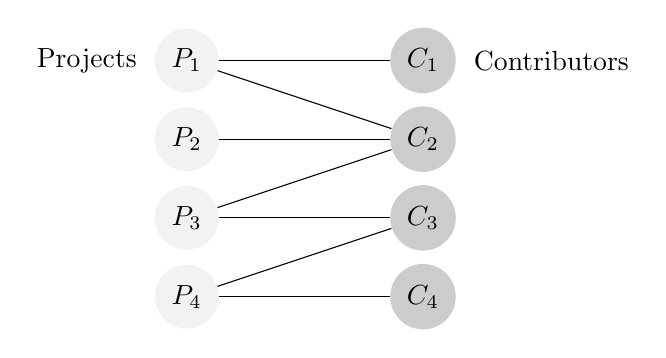
\begin{tikzpicture}
\tikzset{P/.style={circle,fill=lightgray!20}}
\tikzset{C/.style={circle,fill=black!20}}

 [scale=.5,auto=left]
  \node[P] (p1) at (-5,3)  {$P_1$};
  \node[P] (p2) at (-5,2)  {$P_2$};
  \node[P] (p3) at (-5,1)  {$P_3$};
  \node[P] (p4) at (-5,0)  {$P_4$};

  \node[C] (c1) at (-2,3)  {$C_1$};
  \node[C] (c2) at (-2,2)  {$C_2$};
  \node[C] (c3) at (-2,1)  {$C_3$};
  \node[C] (c4) at (-2,0)  {$C_4$};
  
  \draw ({p1}) -- ({c1});
  \draw ({p1}) -- ({c2});
  \draw ({p2}) -- ({c2});;
  \draw ({p3}) -- ({c2});
  \draw ({p3}) -- ({c3});
  \draw ({p4}) -- ({c3});
  \draw ({p4}) -- ({c4});
  \node[draw=none,fill=none,rectangle,left=1mm of p1] {Projects}; 
  \node[draw=none,fill=none,rectangle,right=1mm of c1] {Contributors}; 
\end{tikzpicture}
\caption{An example bipartite graph of Projects and Contributors}
\end{figure}

A bipartite graph projection. in necessary to further analyze the graph. A bipartite projection involves taking the disjoint node sets $P$ and $C$, and representing the graph as relationships between only one of those sets of nodes. A projection onto the project nodes, or $P$, of figure \ref{fig:example_bipartite_graph} is show in figure \ref{fig:example_bipartite_projection_graph}. Here, projects are connected directly, with edges occurring if one or more developer is shared between the projects. It is important to note that the projection could have been done in terms of the contributors, not the projects. This would have led to a graph with nodes of contributors $C$, each being linked by sharing a common project. This approach is another common way of representing these bipartite graphs\cite{newman2001scientific}, and illustrates the fact that a bipartite projections are lossy compared to the data reprented in the original graph\cite{zhou2007bipartite}.\\

One of the main sources of information loss is multiple connections between projects, or projects that share multiple collaborators. When doing a bipartite projection based on projects $P$, a single link could represent one shared developer or many. This is a source of data loss in the projection. The simple approach is to treat one connection the same as many connections between nodes. This is straightforward but lossy\cite{zhou2007bipartite,grossman1995portion}. A better approach is to assign a \textit{weight} to each edge representing repeated links -- or in our case -- multiple shared collaborators\cite{zha2001bipartite,barrat2004architecture}.

\begin{figure}
\label{fig:example_bipartite_projection_graph}
\centering
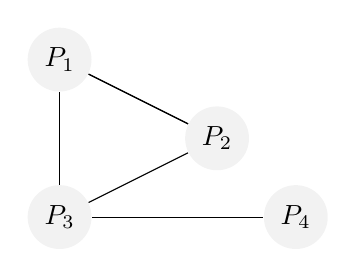
\begin{tikzpicture}
\tikzset{P/.style={circle,fill=lightgray!20}}
\tikzset{C/.style={circle,fill=black!20}}

 [scale=.5,auto=left]
  \node[P] (p1) at (-5,3)  {$P_1$};
  \node[P] (p2) at (-3,2)  {$P_2$};
  \node[P] (p3) at (-5,1)  {$P_3$};
  \node[P] (p4) at (-2,1)  {$P_4$};

  \draw ({p1}) -- ({p3});
  \draw ({p1}) -- ({p2});
  \draw ({p1}) -- ({p2});
  \draw ({p2}) -- ({p3});
  \draw ({p3}) -- ({p4});
\end{tikzpicture}
\caption{A $P$ projection of the figure \ref{fig:example_bipartite_graph} bipartite graph}
\end{figure}

\subsubsection{Graph Analysis}
To support our hypotheses, there are several key metrics to be studied in regards to the aforementioned graph. Many of these metrics follow the work of Boccaletti \textit{et. al}\cite{boccaletti2006complex}, and other studies of similar graph types CITATION HERE.

\textit{Clustering Coefficient (Transitivity)}\\
We calculate the \textit{Clustering Coefficient} (or $C^\Delta$) as a measure of the proportion of closed triangles in a graph\cite{newman2003structure}:
\[C^\delta = 3 \times \frac{\text{number of triangles}}
                    {\text{number of connected triples}}\]

\textit{Clustering Coefficient (Average)}\\
Another approach to clustering is to take the average of each node's local clustering coefficient\cite{watts1998collective}.

\[ c_i = \frac{|\{e_{jk}\}|}{k_i(k_i-1)} :\, v_j,v_k \in N_i,\, e_{jk} \in E \]

{$N_i = \{v_j : e_{ij} \in E\}$}

\textit{Average Path Length}\\
Also, calculating the \textit{Path Length} ($L$) allows us to determine how far removed developers in the graph are from one another. The path length is calculated as the average distance between any two node pairs in the graph:

\[L = \frac{1}{|P| \cdot (|P|-1)} \sum_{i \neq j}\lambda(v_i,v_j)\]

Where {$v_i \in P$}, {$v_j \in P$}, and {$\lambda(v_i,v_j)$} denotes the shortest path between the two nodes. We only consider path length for connected subgraphs, avoiding some complexities of this calculation on disconnected graphs\cite{boccaletti2006complex}.

Results were analyzed using the Python graph processing packaged NetworkX\cite{hagberg-2008-exploring}.

\begin{figure}
\label{fig:example_graphs}
\centering
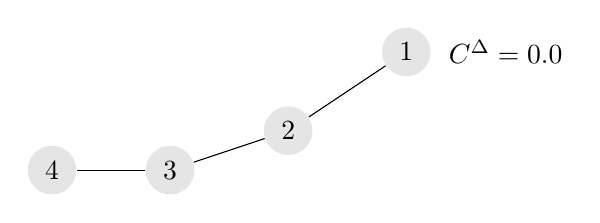
\begin{tikzpicture}
  [scale=.5,auto=left,every node/.style={circle,fill=gray!20}]
  \node (n1) at (15,8) {1};
  \node (n2) at (12,6)  {2};
  \node (n3) at (9,5)  {3};
  \node (n4) at (6,5)  {4};
  \node[draw=none,fill=none,rectangle,right=1mm of n1] {$C^\Delta = 0.0$}; 
  
  \draw ({n1}) -- ({n2});
  \draw ({n2}) -- ({n3});
  \draw ({n3}) -- ({n4});
\end{tikzpicture}

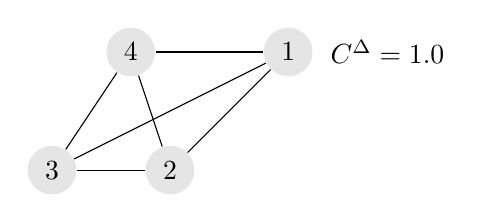
\begin{tikzpicture}
  [scale=.5,auto=left,every node/.style={circle,fill=gray!20}]

  \node (n1) at (15,8) {1};
  \node (n2) at (12,5)  {2};
  \node (n3) at (9,5)  {3};
  \node (n4) at (11,8)  {4};
  \node[draw=none,fill=none,rectangle,right=1mm of n1] {$C^\Delta = 1.0$}; 
  
  \draw ({n1}) -- ({n2});
  \draw ({n2}) -- ({n3});
  \draw ({n3}) -- ({n4});
  \draw ({n1}) -- ({n4});
  \draw ({n1}) -- ({n3});
  \draw ({n2}) -- ({n4});
\end{tikzpicture}

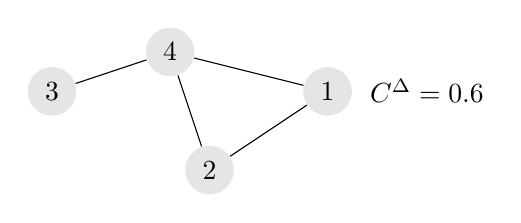
\begin{tikzpicture}
  [scale=.5,auto=left,every node/.style={circle,fill=gray!20}]
  \node (n1) at (15,7) {1};
  \node (n2) at (12,5)  {2};
  \node (n3) at (8,7)  {3};
  \node (n4) at (11,8)  {4};
  \node[draw=none,fill=none,rectangle,right=1mm of n1] {$C^\Delta = 0.6$}; 

  \draw ({n1}) -- ({n2});
  \draw ({n3}) -- ({n4});
  \draw ({n1}) -- ({n4});
  \draw ({n2}) -- ({n4});
\end{tikzpicture}
\caption{A caption.}
\end{figure}



\textit{Small-World-ness}\\

\[\gamma^{\Delta}_g = \frac{C^{\Delta}_g }{C^{\Delta}_{rand} } \]

\[\lambda_g = \frac{L_g }{L_{rand} } \]

\[S^\Delta = \frac{\gamma^{\Delta}_g }{\lambda_g} \]


\subsubsection{Qualitative Analysis}
It has been asserted that people tend to make connections with people with whom they share similarities\cite{mcpherson2001birds}. This idea of homophily, however, needs to be further expanded before we can make assertions about correlations to performance. It has been shown that demographic homophily is complex to measure, correlates little to performance outcomes, and in fact correlate negatively\cite{reagans2004make,lawrence1997perspective}. For our purposes, it is much more appropriate to examine how teams best leverage similarities of knowledge and information, as the flow of these assets can be a key driver to success\cite{nissen2002extended}.
 
\section{Results}

\subsection{Quantitative}

\begin{table}[htbp]\centering
\caption{\label{fig:summary_stats}
\textbf{Statistics} }\begin{tabular} {@{} l r  r  r  r  r  r  @{}} \\ \hline
\textbf{Statistic} & \textbf{Mean} & \textbf{Med} & \textbf{Max} & \textbf{Min} & \textbf{Std} \\ 
\hline
$S^\Delta$ & 1.46 & 1.52 & 4.2 & 0.0 & 0.52 \\ 
Popularity & 63.78 & 41.19 & 3978.95 & 5.12 & 88.81 \\ 
L & 1.01 & 1.0 & 2.4 & 1.0 & 0.07 \\ 
Q & 0.5 & 0.62 & 1.0 & 0.0 & 0.49 \\ 
Edges & 20.64 & 3.0 & 23441.0 & 1.0 & 367.17 \\ 
$C^\Delta$ & 0.51 & 0.82 & 1.0 & 0.0 & 0.5 \\ 
Nodes & 3.88 & 3.0 & 221.0 & 2.0 & 5.86 \\ 
\hline
\multicolumn{6}{@{}l}{
Projects: 41121, Subgraphs: 7172, Contributors: 21970}
\end{tabular}
\end{table}


Summary statistics for the graph analysis are captured in figure \ref{fig:summary_stats}. First, $S^\Delta > 1$ is observed for both the mean and the median, which meets the criteria for a small-world network\cite{humphries2008network}.\\

$Q$ and $C^\Delta$ both indicate a non-normal distribution, as shown by the large standard deviation. This observation indicates a propensity towards the extremes of these measurements. This is further reinforced by the distribution of $Q$ shown in figure \ref{fig:q_distribution}. This figure indicates that the majority of subgraphs have a $Q$ and $C^\Delta$ value of close to either 0 or 1.\\

Exploring this phenomenon further, follows that most graphs resemble the top or the middle graph in figure \ref{fig:example_graphs}, with relatively few resembling the bottom graph.

To validate the hypothesis, we expect to find that medium values of $C^\Delta$ will be correlated with more popular projects. To explore this possibility, we first compare the popularity given $C^\Delta$ values as shown in figure \ref{fig:cc_popular}. The $C^\Delta$ values do display the U-shaped characteristic as compared to popularity, which aligns with the findings of Uzzi \textit{et. al}\cite{uzzi2005collaboration}. It is important to note, however that, the standard deviation is high, as shown in both \ref{fig:summary_stats} and the significant difference between the mean and median results.

\begin{figure}
\label{fig:cc_popular}
\begin{center}
\caption{$C^\Delta$ of Popular Projects}
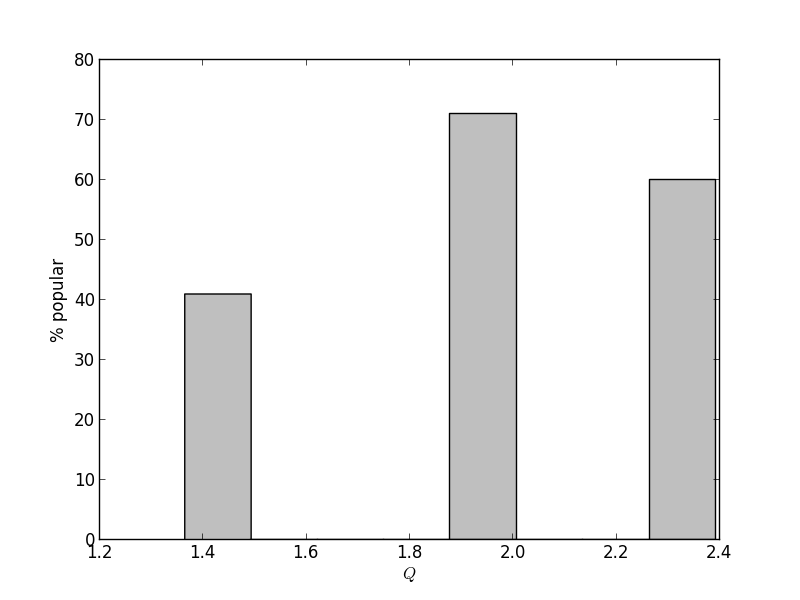
\includegraphics[width=0.5\textwidth]{images/freecode-popular.png}
\end{center}
\end{figure}

\begin{figure}
\begin{center}
\caption{$C^\Delta$ of Unpopular Projects}
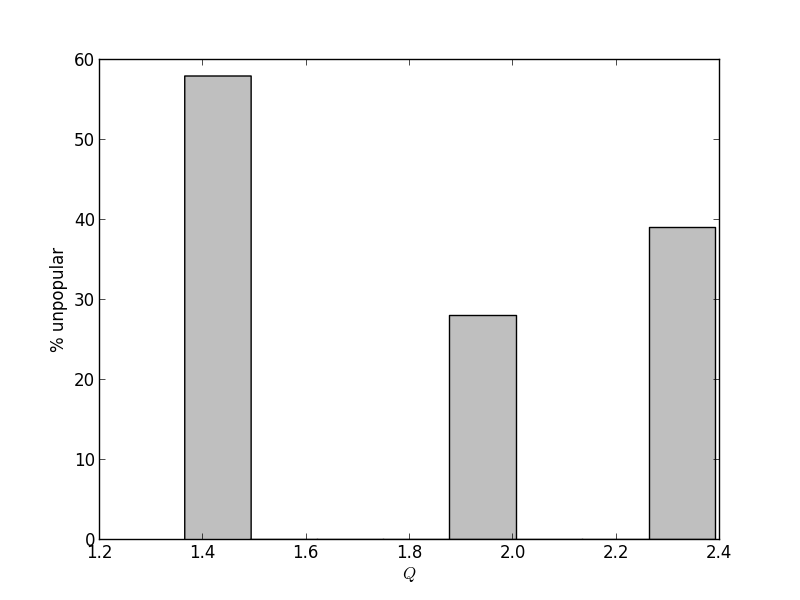
\includegraphics[width=0.5\textwidth]{images/freecode-unpopular.png}
\end{center}
\end{figure}

\begin{figure}
\label{fig:q_distribution}
\begin{center}
\caption{$Q$ Distribution}
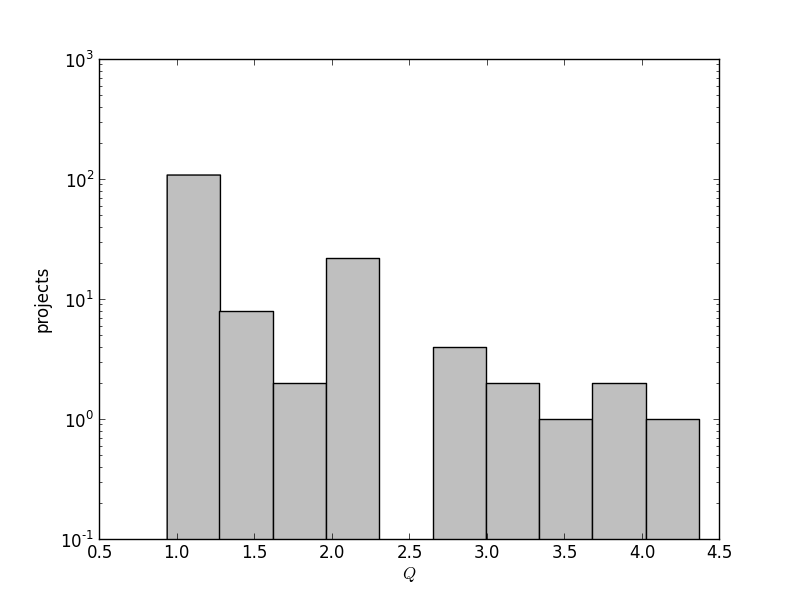
\includegraphics[width=0.5\textwidth]{images/freecode-q-histo.png}
\end{center}
\end{figure}

\begin{figure}
\begin{center}
\caption{$S^\Delta$ Distribution}
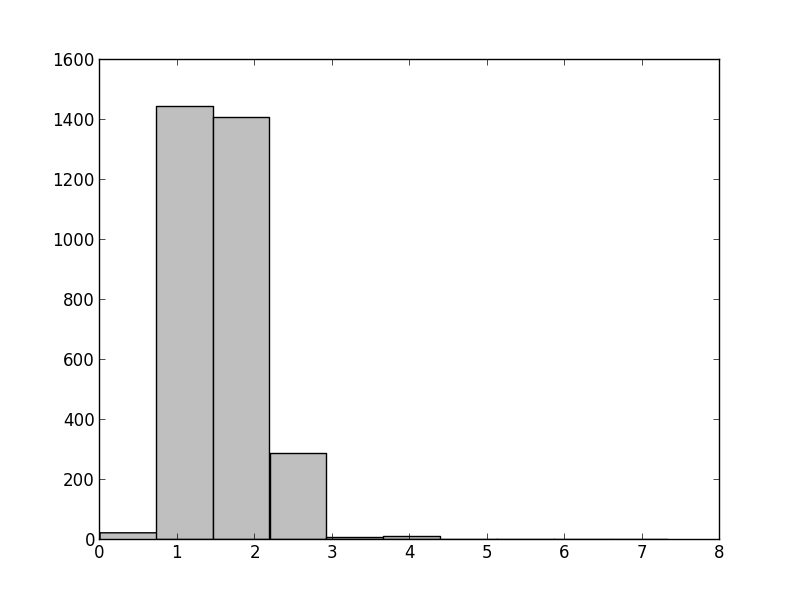
\includegraphics[width=0.5\textwidth]{images/freecode-smallworld-histo.png}
\end{center}
\end{figure}

\begin{figure}
\begin{center}
\caption{$C^\Delta$ and Project Popularity}
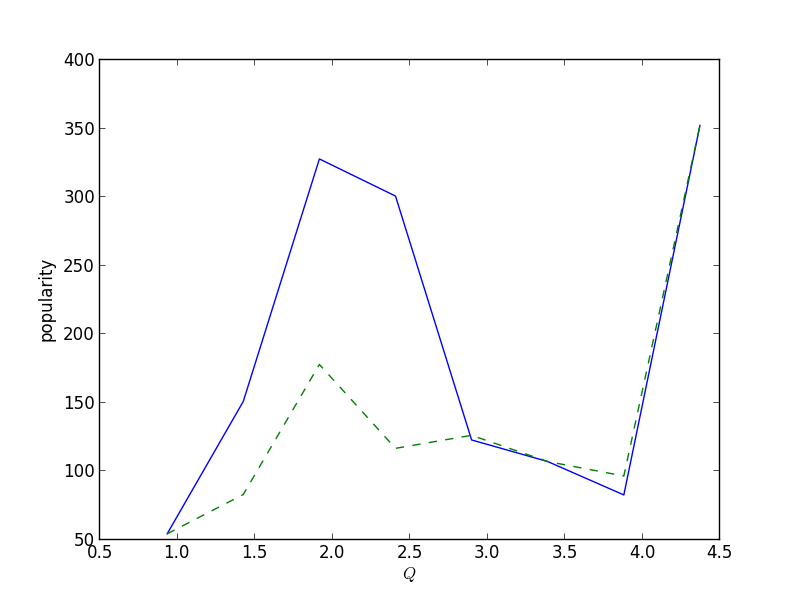
\includegraphics[width=0.5\textwidth]{images/freecode-graph.png}
\end{center}
\end{figure}

The project graph contains a large amount of subgraphs, and as a whole appears less clustered than some other observed social network graphs\cite{madey2002open}.

\subsection{Qualitative}

\section{Conclusion}


\section{Acknowledgments}

\bibliographystyle{plain}
\bibliography{bibliography}


\end{document}